\documentclass[fontset=windows]{article}
\usepackage[margin=1in]{geometry}%设置边距,符合Word设定
\usepackage[UTF8]{ctex}
\usepackage{setspace}
\usepackage{amsmath}
\numberwithin{figure}{section}
\usepackage{array}
\usepackage{lipsum}
\usepackage{float}
\usepackage{graphicx}%插入图片
\usepackage[dvipsnames]{xcolor}
\usepackage{authblk}
\usepackage{listings,matlab-prettifier}
\lstset{
	language=Matlab, % 设置代码语言为Matlab
    basicstyle=\ttfamily, % 设置字体为等宽字体
    numbers=left, % 行号在左边显示
    numberstyle=\tiny, % 设置行号字体大小
    stepnumber=1, % 行号递增步长
    numbersep=5pt, % 行号到代码的距离
    backgroundcolor=\color{gray!10}, % 设置代码的背景颜色
    showspaces=false,
    showstringspaces=false,
    showtabs=false,
    frame=single, % 设置代码框
    rulecolor=\color{black},
    tabsize=2,
    breaklines=true,
    breakatwhitespace=true,
    title=\lstname,
	keywordstyle=\bfseries\color{NavyBlue},
	morekeywords={var,};
	emphstyle=\bfseries\color{Rhodamine}, % 强调词样式设置
    commentstyle=\itshape\color{black!50!white}, % 设置注释样式,斜体,浅灰色
    stringstyle=\bfseries\color{PineGreen!90!black}, % 设置字符串样式
	columns=flexible,
}
\graphicspath{{Figures1/}}%文章所用图片在当前目录下的 Figures目录

\usepackage{hyperref} % 对目录生成链接,注:该宏包可能与其他宏包冲突,故放在所有引用的宏包之后
\hypersetup{colorlinks = true,  % 将链接文字带颜色
	linkcolor=black, % 将链接文字黑色
	bookmarksopen = true, % 展开书签
	bookmarksnumbered = true, % 书签带章节编号
	} % 作者
\bibliographystyle{plain}% 参考文献引用格式

\renewcommand{\contentsname}{\centerline{目录}} %经过设置word格式后,将目录标题居中

\title{\heiti\zihao{2} 《统计信号处理》第一教学单元研讨题}
\author{杨 鼎,韦可雷,高司博,高涵博}
\date{}

\begin{document}
\maketitle
\thispagestyle{empty}

%\begin{abstract}
%	\lipsum[2]
%\end{abstract}

\tableofcontents
\setcounter{page}{0}
\newpage

\section{第一题}
对于矢量形式的线型模型 \(\mathbf{z=H}\boldsymbol{\theta}+\mathbf{w}\) ,其中 \(\mathbf{w}\) 为高斯序列,
\(PDF\)为\(N(\mathbf{0,\sigma^2I})\),(1)试问有效估计量是否存在?CRLB等于多少?
如果有效估计量存在,该估计量服从什么分布?(2)对于观测模型:z[n]=A+B·n+w[n]
,n=0,1,…,N-1,其中w[n]是零均值高斯白噪声,方差为\(\sigma^2\),A和B为待估计参数,
试将此问题转化为线性模型,确定模型的各参数,并求出有效估计量及估计的方差阵。

\subsection*{(1)有效估计量是否存在?}

已知矢量线性模型\(\mathbf{z=H}\boldsymbol{\theta}+\mathbf{w}\),其中\(\mathbf{w}\sim \mathcal{N} (0,\sigma^2 \mathbf{I})\)
,则有

\begin{align*}
	p(\mathbf{z};\boldsymbol{\theta})=(\frac{1}{2\pi \sigma^2})^{\frac{N}{2}}
	\exp\left[-\frac{1}{2\sigma^2}(\mathbf{z-H\boldsymbol{\theta}})^T
		(\mathbf{z-H\boldsymbol{\theta}})\right]
\end{align*}

对数似然函数

\begin{align*}
	\ln p(\mathbf{z};\boldsymbol{\theta})=-{\frac{N}{2}}\ln (2\pi \sigma^2)
	-\frac{1}{2\sigma^2}(\mathbf{z-H}\boldsymbol{\theta})^T(\mathbf{z-H}\boldsymbol{\theta})
\end{align*}

对\(\boldsymbol{\theta}\)求导有

\begin{align*}
	\frac{\partial \ln p(\mathbf{z};\boldsymbol{\theta})}{\partial \boldsymbol{\theta}}
	 & =\frac{\partial}{\partial \boldsymbol{\theta}}\left[-\frac{1}{2\sigma^2}
	(\mathbf{z-H}\boldsymbol{\theta})^T(\mathbf{z-H}\boldsymbol{\theta})\right]                               \\
	 & = -\frac{1}{2\sigma^2}\frac{\partial}{\partial \boldsymbol{\theta}}\left(\mathbf{z}^T\mathbf{z}
	-\mathbf{z}^T\mathbf{H}\boldsymbol{\theta}-\boldsymbol{\theta}^T\mathbf{H}^T\mathbf{z}+
	\boldsymbol{\theta}^T\mathbf{H}^T\mathbf{H}\boldsymbol{\theta}\right)                                     \\
	 & =-\frac{1}{2\sigma^2}\left(-2\mathbf{H}^T\mathbf{z}+2\mathbf{H}^T\mathbf{H}\boldsymbol{\theta} \right) \\
	 & =\frac{1}{\sigma^2}\left(\mathbf{H}^T\mathbf{z}-\mathbf{H}^T\mathbf{H}\boldsymbol{\theta} \right)
\end{align*}

若存在有效估计量\(\hat{\boldsymbol{\theta}}\),即\(\hat{\boldsymbol{\theta}}\)无偏且方差达到CRLB,由课本定理3.2,则当且仅当

\begin{align*}
	\frac{\partial \ln p(\mathbf{z};\boldsymbol{\theta})}{\partial \boldsymbol{\theta}}=
	\mathbf{I}(\hat{\boldsymbol{\theta}})(\hat{\boldsymbol{\theta}}-\boldsymbol{\theta})
\end{align*}

成立,假定\((\mathbf{H}^T\mathbf{H})^{-1}\)可逆,于是

\begin{align*}
	\frac{\partial \ln p(\mathbf{z};\boldsymbol{\theta})}{\partial \mathbf{\boldsymbol{\theta}}}=
	\frac{\mathbf{H}^T\mathbf{H}}{\sigma^2}\left[\left(\mathbf{H}^T\mathbf{H}\right)^{-1}
		\mathbf{H}^T\mathbf{z}-\theta\right]
\end{align*}

因此易知\(\mathbf{I}(\theta)=\frac{\mathbf{H}^T\mathbf{H}}{\sigma^2}\),
即\(CRLB=\mathbf{I}^{-1}(\theta)=\left(\mathbf{H}^T\mathbf{H}\right)^{-1}\sigma^2\),
有效估计量也存在,\(\theta=\left(\mathbf{H}^T\mathbf{H}\right)\mathbf{H}^T\mathbf{z},
\hat{\boldsymbol{\theta}} \sim \mathcal{N} (\boldsymbol{\theta},
\left(\mathbf{H}^T\mathbf{H}\right)^{-1}\sigma^2)\),

\begin{align*}
	\left[\mathbf{I}(\theta)\right]_{ij}
	 & =-E\left[\frac{\partial^2 \ln p(\mathbf{z};\boldsymbol{\theta})}{\partial \theta_i \partial \theta_j}\right] \\
	 & =\frac{1}{\sigma^2}\frac{\partial}{\partial \theta}\left(-\mathbf{H}^T\mathbf{H}\theta\right)                \\
	 & =-\frac{\mathbf{H}^T\mathbf{H}}{\sigma^2}                                                                    \\
\end{align*}

所以

\begin{align*}
	\mathbf{I}(\theta)=
	-E\left[\frac{\partial^2 \ln p(\mathbf{z};\theta)}{\partial \theta_i \partial \theta_j}\right]
	=-E\left[-\frac{\mathbf{H}^T\mathbf{H}}{\sigma^2}\right]
	=\frac{\mathbf{H}^T\mathbf{H}}{\sigma^2}
\end{align*}

\subsection*{(2)将观测模型转化为线性模型}

将\(z[n]=A+Bn+w[n],n=0,1,…,N-1\)转化为\(\mathbf{z}=\mathbf{H}\boldsymbol{\theta}+\mathbf{w}\),易知

\begin{align*}
	\theta     & =
	\begin{bmatrix}
		A & B
	\end{bmatrix}^T \\
	\mathbf{H} & =
	\begin{bmatrix}
		1 & 1 & 1 & … & 1   \\
		0 & 1 & 2 & … & N-1
	\end{bmatrix}^T
\end{align*}

似然函数

\begin{align*}
	p(\mathbf{z};\boldsymbol{\theta})=(\frac{1}{2\pi \sigma^2})^{\frac{N}{2}}
	\exp\left\{-\frac{1}{2\sigma^2}\left[z[n]-A-Bn\right]\right\}
\end{align*}

\begin{align*}
	\ln p(\mathbf{z};\boldsymbol{\theta})=-{\frac{N}{2}}\ln (2\pi \sigma^2)
	-\frac{1}{2\sigma^2}\sum_{n=0}^{N-1}\left(z[n]-A-Bn\right)^2
\end{align*}

求导有

\begin{align*}
	\frac{\partial \ln p}{\partial A}
	 & =\frac{1}{\sigma^2}\sum_{n=0}^{N-1}\left(z[n]-A-Bn\right)  \\
	\frac{\partial \ln p}{\partial B}
	 & =\frac{1}{\sigma^2}\sum_{n=0}^{N-1}\left(z[n]-A-Bn\right)n \\
	\frac{\partial^2 \ln p}{\partial A^2}
	 & =-\frac{N}{\sigma^2}                                       \\
	\frac{\partial^2 \ln p}{\partial B^2}
	 & =-\frac{1}{\sigma^2}\sum_{n=0}^{N-1}n^2
	=-\frac{1}{\sigma^2}\frac{N(N-1)(2n-1)}{6}                    \\
	\frac{\partial^2 \ln p}{\partial A \partial B}
	 & =-\frac{1}{\sigma^2}\sum_{n=0}^{N-1}n
	=-\frac{1}{\sigma^2}\frac{N(N-1)}{2}
\end{align*}

因此Fisher信息矩阵为

\begin{align*}
	\mathbf{I}(\boldsymbol{\theta})=
	\begin{bmatrix}
		-E[\frac{\partial^2 \ln p}{\partial A^2}]          & -E[\frac{\partial^2 \ln p}{\partial A\partial B}] \\
		-E[\frac{\partial^2 \ln p}{\partial B \partial A}] & -E[\frac{\partial^2 \ln p}{\partial B^2}]
	\end{bmatrix}
\end{align*}

因为二阶导数均与z无关,所以

\begin{align*}
	\mathbf{I}(\boldsymbol{\theta})=
	\begin{bmatrix}
		\frac{N}{\sigma^2}                 & \frac{1}{\sigma^2}\frac{N(N-1)}{2}       \\
		\frac{1}{\sigma^2}\frac{N(N-1)}{2} & \frac{1}{\sigma^2}\frac{N(N-1)(2N-1)}{6}
	\end{bmatrix}
\end{align*}

逆矩阵为

\begin{align*}
	\mathbf{I}^{-1}(\theta)=\sigma^2
	\begin{bmatrix}
		\frac{2(2N-1)}{N(N+1)} & -\frac{6}{N(N+1)}   \\
		-\frac{6}{N(N+1)}      & \frac{12}{N(N^2-1)}
	\end{bmatrix}
\end{align*}

所以

\begin{align*}
	var(\hat{A})=\frac{2(2N-1)\sigma^2}{N(N+1)}
\end{align*}
\begin{align*}
	var(\hat{B})=\frac{12\sigma^2}{N(N^2-1)}
\end{align*}

根据,由定理3.2可知

\begin{align*}
	\frac{\partial \ln p(\mathbf{z};\boldsymbol{\theta})}{\partial \boldsymbol{\theta}}=
	\mathbf{I}(\hat{\boldsymbol{\theta}})(\hat{\boldsymbol{\theta}}-\boldsymbol{\theta})
\end{align*}

有

\begin{align*}
	\frac{\partial \ln p(\mathbf{z};\theta)}{\partial \theta}=	\begin{bmatrix}
		\frac{N}{\sigma^2}                 & \frac{1}{\sigma^2}\frac{N(N-1)}{2}       \\
		\frac{1}{\sigma^2}\frac{N(N-1)}{2} & \frac{1}{\sigma^2}\frac{N(N-1)(2N-1)}{6}
	\end{bmatrix}
	\begin{bmatrix}
		\hat{A}-A \\
		\hat{B}-B
	\end{bmatrix}
\end{align*}

解得有效估计量

\begin{align*}
	\hat{A}=\frac{2(2N-1)}{N(N+1)}\sum_{n=0}^{N-1}z[n]-\frac{6}{N(N+1)}\sum_{n=0}^{N-1}nz[n]
\end{align*}
\begin{align*}
	\hat{B}=-\frac{6}{N(N+1)}\sum_{n=0}^{N-1}z[n]+\frac{12}{N(N^2-1)}\sum_{n=0}^{N-1}nz[n]
\end{align*}

方差阵\(\mathbf{C}_{\theta}=\mathbf{I}^{-1}(\boldsymbol{\theta})\)

\section{第二题}
假定z[n]=A+W[n],其中w[n]是零均值高斯白噪声,(1)方差 \(\sigma^2\)为已知量
A的估计量为\(\hat{A}=\frac{1}{N}\sum_{n = 0}^{N-1}z[n] \),试用蒙特卡
洛仿真的方法分析估计量的性能(估计量的均值、方差、PDF)。(2)如果A和 \(\sigma^2\)
均未知,A和\(\sigma^2\)的估计量分别为\(\hat{A}=\frac{1}{N}\sum_{n=0}^{N-1}z[n]\)
、\(\sigma^2=\frac{1}{N}\sum_{n=0}^{N-1}(z[n]-\frac{1}{N}\sum_{n=0}^{N-1}z[n])^2\)
,试用蒙特卡洛仿真的方法分析估计量的性能(估计量的均值、方差、PDF),并讨论估计量的性能
随N的变化趋势。

\subsection*{(1)估计量\(\hat{A}\)的性能}

\begin{lstlisting}
close all
sigma2=1;%假设方差为1
sigma=sqrt(sigma2);
A=0.1;%预设A为0.1
N=1000;%每组观测产生N个z
M=1000;%共进行M组观测
%%
%进行蒙特卡洛模拟实验,M次观测
A_est=zeros(1,M);
for s=1:M
	a_est=observe(N,A,sigma);%产生一组观测
	A_est(1,s)=a_est;
end
expect_A=mean(A_est);%期望
variance_A=var(A_est);%方差
fprintf('估计量A期望为%1.5f,方差为%2.5f\n',expect_A,variance_A)

%使用正态分布估计参数
params=mle(A_est,'distribution','normal');
A_mle_mu=params(1);
A_mle_sigma=params(2);

figure
his=histogram(A_est,NumBins=50);
yyaxis right
x=linspace(0,max(A_est),200);
pdf=plot(x,1/(sqrt(2*pi)*A_mle_sigma)*exp(-(x-A_mle_mu).^2/(2*A_mle_sigma^2)));
title(['估计量A的概率密度函数,均值为' num2str(A_mle_mu) ',标准差为' num2str(A_mle_sigma)])
xlabel('A取值')
yyaxis left
ylabel('蒙特卡罗仿真计数')
yyaxis right
ylabel('密度函数估计分布')
set(gcf,'unit','normalized','position',[0.2,0.2,0.5,0.33])
%%
% 定义观测函数observe
function a_est=observe(N,A,sigma)
a_est=0;%一次估计量
for i=1:N
	z=A+sigma*randn;%得到z的1次抽样结果
	a_est=a_est+z;
end
a_est=a_est/N;%计算1次抽样的估计量
end
\end{lstlisting}
进行一次仿真计算,得到\(E[\hat{A}]=0.09941\),\(var(\hat{A})=0.00095\),
PDF仿真结果如图2.1。
\begin{figure}[H]
	\centering
	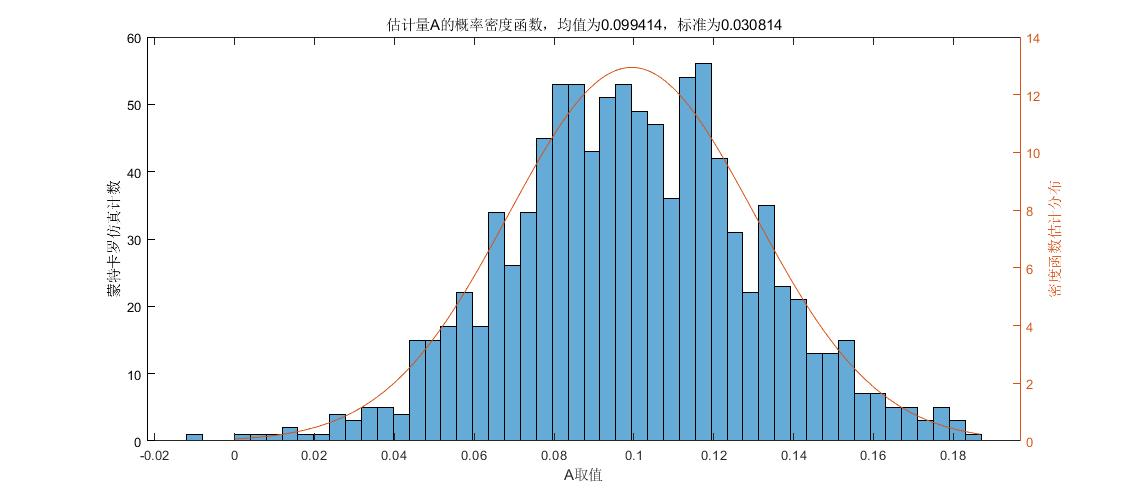
\includegraphics[scale=0.4]{fig2.1.jpg}
	\caption{估计量\(\hat{A}\)的PDF}
	\label{2.1}
\end{figure}

\subsection*{(2)估计量\(\hat{A}\)和\(\sigma^2\)的性能}

\begin{lstlisting}
close all
sigma2=1;%假设方差为1
sigma=sqrt(sigma2);
A=0.1;%预设A为0.1
N=1000;%每组观测产生N个z
M=1000;%共进行M组观测
%%
%进行蒙特卡洛模拟实验,M次观测
A_est=zeros(1,M);
Sigma2_est=zeros(1,M);
for s=1:M
	[a_est,sigma2_est]=observe(N,A,sigma);%产生一组观测
	A_est(1,s)=a_est;
	Sigma2_est(1,s)=sigma2_est;
end
%%
%分析估计量A
expect_A=mean(A_est);%期望
variance_A=var(A_est);%方差
fprintf('估计量A期望为%1.5f,方差为%2.5f\n',expect_A,variance_A)

%使用正态分布估计A服从分布的参数
params_A=mle(A_est,'distribution','normal');
A_mle_mu=params_A(1);
A_mle_sigma=params_A(2);

figure
his_A=histogram(A_est,NumBins=50);
yyaxis right
x=linspace(min(A_est),max(A_est),200);
pdf_A=plot(x,1/(sqrt(2*pi)/A_mle_sigma)*exp(-(x-A_mle_mu).^2/(2*A_mle_sigma^2)));
title(['估计量A的概率密度函数,均值为' num2str(A_mle_mu) ',标准为' num2str(A_mle_sigma)])
xlabel('A取值')
yyaxis left
ylabel('蒙特卡罗仿真计数')
yyaxis right
ylabel('密度函数估计分布')
set(gcf,'unit','normalized','position',[0.2,0.2,0.5,0.33])
%%
%分析估计量Sigma2
expect_sigma=mean(Sigma2_est);%期望
variance_sigma=var(Sigma2_est);%方差
fprintf('估计量期望sigma2为%1.5f,方差为%2.5f\n',expect_sigma,variance_sigma)

%使用正态分布估计sigma2服从分布的参数
params_sigma=mle(Sigma2_est,'distribution','normal');
sigma2_mle_mu_est=params_sigma(1);
sigma2_mle_sigma=params_sigma(2);

figure
his_sigma2=histogram(Sigma2_est,NumBins=50);
yyaxis right
x=linspace(min(Sigma2_est),max(Sigma2_est),200);
pdf_sigma2=plot(x,1/(sqrt(2*pi)/sigma2_mle_sigma)*exp(-(x-sigma2_mle_mu_est).^2/...
	(2*sigma2_mle_sigma^2)));
title(['估计量sigma2的概率密度函数,均值为' num2str(sigma2_mle_mu_est) ',标准为' num2str(sigma2_mle_sigma)])
xlabel('sigma2取值')
yyaxis left
ylabel('蒙特卡罗仿真计数')
yyaxis right
ylabel('密度函数估计分布')
set(gcf,'unit','normalized','position',[0.2,0.6,0.5,0.33])
%%
% 定义观测函数observe
function [a_est,sigma_est]=observe(N,A,sigma)
Z=zeros(1,N);
for n=1:N
	z=A+sigma*randn;%得到z的1次抽样结果
	Z(1,n)=z;
end
a_est=sum(Z)/N;%计算1次观测的A估计量
sigma_est=sum((Z-a_est).^2)/N;
end
\end{lstlisting}

进行一次仿真计算,得到\(E[\hat{A}]=0.10055\),\(var(\hat{A})=0.00093\)。
估计量\(\hat{A}\)的PDF仿真结果如图2.2。
\begin{figure}[H]
	\centering
	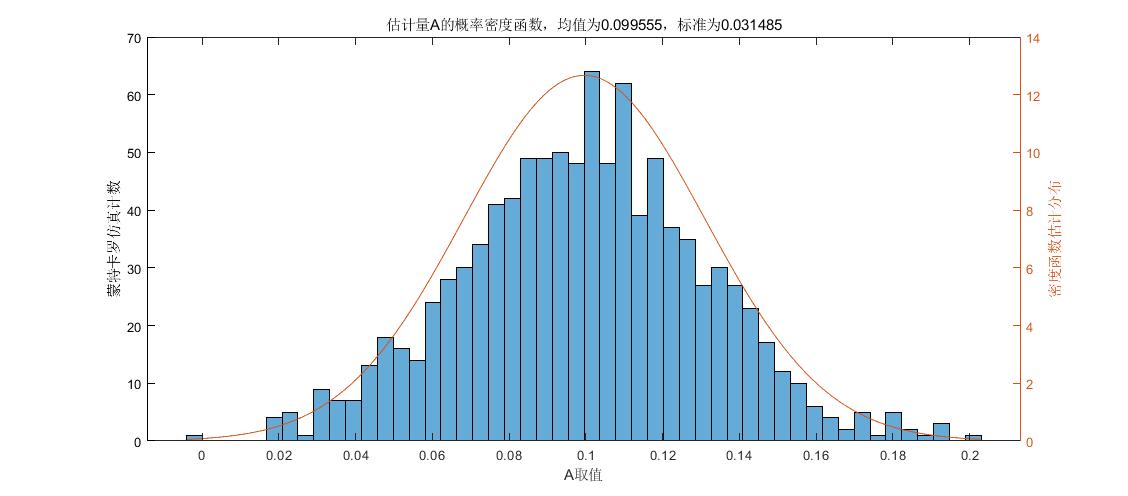
\includegraphics[scale=0.4]{fig2.2.jpg}
	\caption{估计量\(\hat{A}\)的PDF}
	\label{2.2}
\end{figure}

得到\(E[\sigma^2]=1.00011\),\(var(\sigma^2)=0.00196\)。
估计量\(\sigma^2\)的PDF仿真结果如图2.3。
\begin{figure}[H]
	\centering
	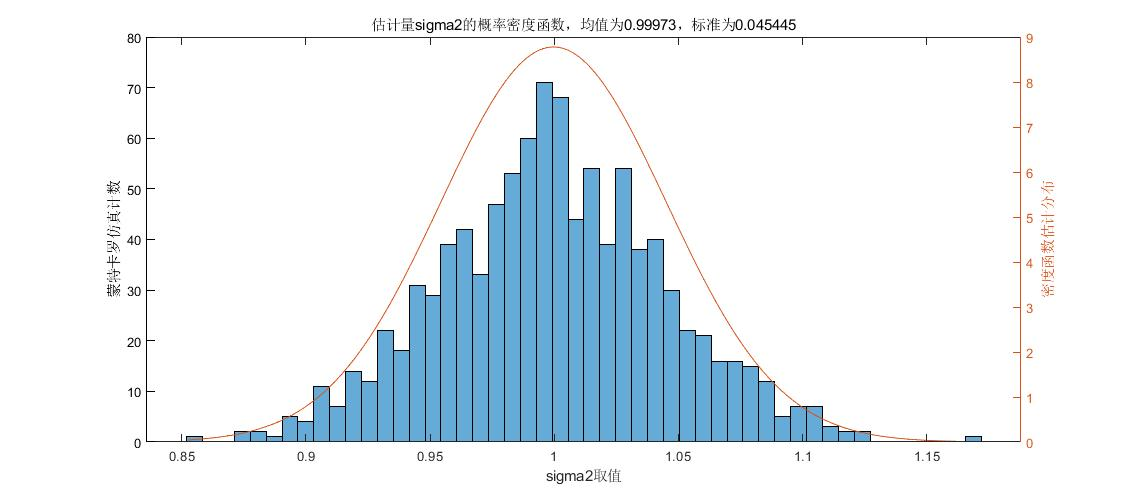
\includegraphics[scale=0.4]{fig2.3.jpg}
	\caption{估计量\(\sigma^2\)的PDF}
	\label{2.3}
\end{figure}

\subsection*{(3)估计量性能随N的变化讨论}

\begin{lstlisting}
close all
sigma2=1;%假设方差为1
sigma=sqrt(sigma2);
A=0.1;%预设A为0.1
N=1000;%每组观测产生N个z
M=1000;%共进行M组观测
%%
%记录估计量A的期望、方差,估计量sigma2的期望、方差,随N的变化
Expect_A=zeros(1,N);%期望
Variance_A=zeros(1,N);%方差

Expect_sigma=zeros(1,N);%期望
Variance_sigma=zeros(1,N);%方差

for i=1:N
	[expect_A,variance_A,expect_sigma,variance_sigma]=MonteCralo(M,i,A,sigma);
	%进行一次蒙特卡洛仿真
	
	%记录一次仿真结果
	Expect_A(1,i)=expect_A;
	Variance_A(1,i)=variance_A;
	
	Expect_sigma(1,i)=expect_sigma;
	Variance_sigma(1,i)=variance_sigma;
end

figure
x=linspace(1,N,N);
Exp_A=plot(x,Expect_A);
yyaxis right
Exp_sigma=plot(x,Expect_sigma);
title('N从1至1000,估计量A和sigm2的期望变化曲线')
xlabel('N')
yyaxis left
ylabel('估计量A的期望变化曲线')
yyaxis right
ylabel('估计量sigma2的期望变化曲线')
set(gcf,'unit','normalized','position',[0.2,0.6,0.5,0.33])

figure
Var_A=plot(x,log(Variance_A));
yyaxis right
Var_sigma=plot(x,log(Variance_sigma));
title('N从1至1000,估计量A和sigma2的方差对数log(var)变化曲线')
xlabel('N')
yyaxis left
ylabel('估计量A的方差对数变化曲线')
yyaxis right
ylabel('估计量sigma2的方差对数变化曲线')
set(gcf,'unit','normalized','position',[0.2,0.2,0.5,0.33])
%%
% 定义观测函数observe
function [a_est,sigma_est]=observe(N,A,sigma)
Z=zeros(1,N);
for n=1:N
	z=A+sigma*randn;%得到z的1次抽样结果
	Z(1,n)=z;
end
a_est=sum(Z)/N;%计算1次观测的A估计量
sigma_est=sum((Z-a_est).^2)/N;
end
%%
% 定义蒙特卡洛仿真函数,即以N次抽样作为一组观测,以M次观测作为计算一次仿真结果
function [expect_A,variance_A,expect_sigma,variance_sigma]=MonteCralo(M,N,A,sigma)
A_est=zeros(1,M);
Sigma_est=zeros(1,M);
for s=1:M
	[a_est,sigma_est]=observe(N,A,sigma);%产生一组观测
	A_est(1,s)=a_est;
	Sigma_est(1,s)=sigma_est;
end
expect_A=mean(A_est);%期望
variance_A=var(A_est);%方差
expect_sigma=mean(Sigma_est);%期望
variance_sigma=var(Sigma_est);%方差
end
\end{lstlisting}

当N从1至1000变化时,估计量\(\hat{A}\)和估计量\(\sigma^2\)的期望变化如图2.4。
\begin{figure}[H]
	\centering
	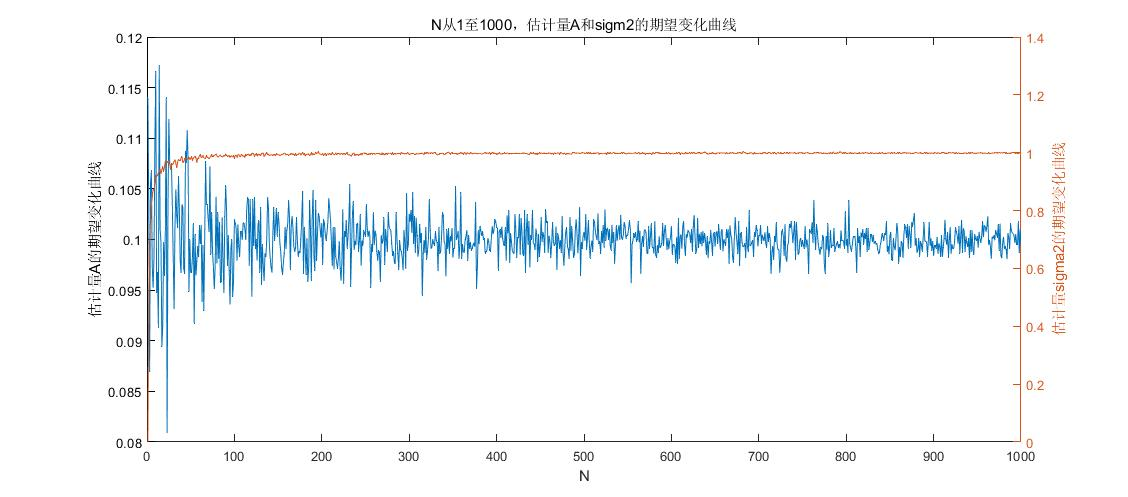
\includegraphics[scale=0.4]{fig2.4.jpg}
	\caption{估计量\(\hat{A}\)和\(\sigma^2\)的期望随N增长的变化曲线}
	\label{2.4}
\end{figure}
从图2.4中可以看出,当N等于1000时,估计量\(\hat{A}\)和\(\sigma^2\)的期望接近于各自真值,
这说明从无偏性角度来看,估计量\(\hat{A}\)和\(\sigma^2\)都应当都是无偏估计。

当N从1至1000变化时,估计量\(\hat{A}\)和估计量\(\sigma^2\)的方差的自然对数
(即ln(var(\(\hat{A}\)))和ln(var(\(\sigma^2\))))变化如图2.5。

\begin{figure}[H]
	\centering
	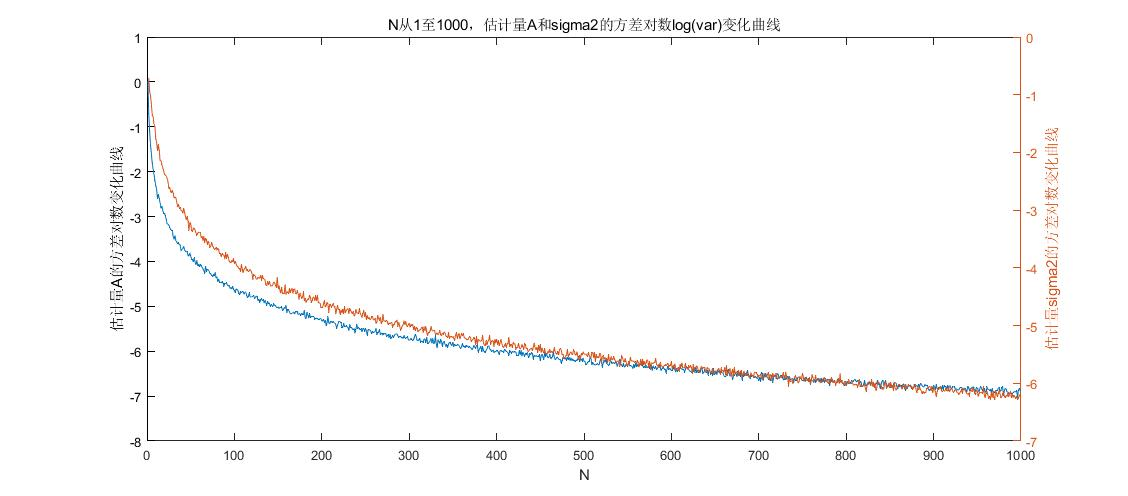
\includegraphics[scale=0.4]{fig2.5.jpg}
	\caption{估计量\(\hat{A}\)和\(\sigma^2\)的方差自然对数ln(var)随N增长的变化曲线}
	\label{2.5}
\end{figure}

由于估计量\(\hat{A}\)和估计量\(\sigma^2\)的收敛速度均较快,为对比明显起见,
图2.5中纵轴均取估计量方差的自然对数。从图2.5可以看出,随着N的增大,
估计量\(\hat{A}\)和估计量\(\sigma^2\)的方差均逐渐减小,且收敛速度接近。
这说明从有效性角度来看,估计量\(\hat{A}\)和估计量\(\sigma^2\)有效性接近。

\section{第三题}
假定雷达接收信号可以表示为\(s=Acos(2\pi fn+\varphi)+w(n),n=1,…,N\),N为观测次数
,\(w(n)\sim\mathcal{N}(0,\sigma^2)\)。

(1)A、\(\sigma^2\)已知,均为确定参数,\(f\)未知,\(0<f<\frac{1}{2}\)。试推导\(f\)估计的CRLB
,采用MATLAB画出CRLB随频率、信噪比 、观测次数的变化曲线。

(2)若A、\(\varphi\)、\(f\)均未知,试推导\(f\)估计的CRLB,采用MATLAB画出CRLB随其影响参数的
变化曲线。并对比分析此时\(f\)估计方差的CRLB与第(1)问中\(f\)估计方差的CRLB。

(3)若噪声\(w(n)\)服从瑞利分布,噪声平均功率与高斯分布情况下相同,试再次分析
第(1)、(2)问中参数估计的CRLB。并分析导致CRLB差异的原因。

\subsection*{(1) A、\(\sigma^2\)已知,均为确定参数,\(f\)未知}

已知\(x[n]=s[n;\theta]+w[n]\),其中\(s=Acos(2\pi f n +\varphi + w(n))\),
n=1,…,N,\(w(n)\sim \mathcal{N} (0,\sigma^2)\)。极大似然函数

\begin{align*}
	p(\mathbf{x};\theta)=(\frac{1}{2\pi \sigma^2})^{\frac{N}{2}}
	\exp\{ -\frac{1}{2\sigma^2}\sum_{n=0}^{N-1}(x[n]-s[n;\theta])^2 \}
\end{align*}
一次求导得到
\begin{align*}
	\frac{\partial p(\mathbf{x};\theta)}{\partial \theta}=
	\frac{1}{\sigma^2}\sum_{n=0}^{N-1}(x[n]-s[n;\theta])\frac{\partial s[n;\theta]}{\partial\theta}
\end{align*}
二次求导得到
\begin{align*}
	\frac{\partial^2 p(\mathbf{x};\theta)}{\partial \theta}=
	\frac{1}{\sigma^2}\sum_{n=0}^{N-1}\{(x[n]-s[n;\theta])
	\frac{\partial^2 s[n;\theta]}{\partial\theta^2}
	-\left(\frac{s[n;\theta]}{\theta}\right)^2\}
\end{align*}
取数学期望后得到
\begin{align*}
	E\left(\frac{\partial^2 p(\mathbf{x};\theta)}{\partial \theta}\right)=
	-\frac{1}{\sigma^2}\sum_{n=0}^{N-1}
	\left(\frac{s[n;\theta]}{\theta}\right)^2
\end{align*}
将\(s=Acos(2\pi f n +\varphi + w(n))\)带入得到
\begin{align*}
	E\left(\frac{\partial^2 p(\mathbf{x};\theta)}{\partial \theta}\right)=
	-\frac{A^2}{\sigma^2}\sum_{n=0}^{N-1}
	\left[2\pi f n \sin(2\pi f n+\varphi)\right]^2
\end{align*}
得到CRLB为
\begin{align*}
	var(\hat{f})
	\geq \frac{\sigma^2}{A^2 \sum_{n=0}^{N-1}
		\left[2\pi f n \sin(2\pi f n+\varphi)\right]^2}
	=	\frac{1}{\eta ^2 \sum_{n=0}^{N-1}
		\left[2\pi f n \sin(2\pi f n+\varphi)\right]^2}
\end{align*}

\subsection*{(2) A、\(\varphi\)、\(f\)均未知}
如果A、\(\varphi\)、\(f\)均未知,估计量\(\boldsymbol{\theta}=[Af\phi]^T\),由于

\begin{align*}
	[\mathbf{I}(\boldsymbol{\theta})]_{ij}=\frac{1}{\sigma^2}\sum_{n=0}^{N-1}
	\frac{\partial s[n;\boldsymbol{\theta}]}{\partial \theta_i}
	\frac{\partial s[n;\boldsymbol{\theta}]}{\partial \theta_j}
\end{align*}

如果\(f\)不靠近0或者1/2,对于\(i=0,1,2\)

\begin{align*}
	\frac{1}{N^{i+1}}\sum_{n=0}^{N-1}n^i\sin(4\pi f n+2\varphi)\approx 0 \\
	\frac{1}{N^{i+1}}\sum_{n=0}^{N-1}n^i\cos(4\pi f n+2\varphi)\approx 0
\end{align*}

利用近似,并且令\(\alpha=2\pi fn+\varphi\),得到

\begin{align*}
	[\mathbf{I}(\boldsymbol{\theta})]_{11}
	 & =\frac{1}{\sigma^2}\sum_{n=0}^{N-1}\cos^2 \alpha
	=\frac{1}{\sigma^2}\sum_{n=0}^{N-1}\left(\frac{1}{2}-\frac{1}{2}\cos2\alpha\right)
	\approx\frac{N}{2\sigma^2}                                           \\
	[\mathbf{I}(\boldsymbol{\theta})]_{12}
	 & =-\frac{1}{\sigma^2}\sum_{n=0}^{N-1}A2\pi n \cos\alpha \sin\alpha
	=-\frac{\pi A}{\sigma^2}\sum_{n=0}^{N-1}n\sin 2\alpha
	\approx 0                                                            \\
	[\mathbf{I}(\boldsymbol{\theta})]_{13}
	 & =-\frac{1}{\sigma^2}\sum_{n=0}^{N-1}A\cos\alpha \sin\alpha
	=-\frac{A}{2\sigma^2}\sum_{n=0}^{N-1}\sin 2\alpha
	\approx 0                                                            \\
	[\mathbf{I}(\boldsymbol{\theta})]_{22}
	 & =\frac{1}{\sigma^2}\sum_{n=0}^{N-1}A^2(2\pi n)^2\sin^2 \alpha
	=\frac{(2\pi A)^2}{\sigma^2}\sum_{n=0}^{N-1}n^2\left(\frac{1}{2}-
	\frac{1}{2}\cos2\alpha\right)                                        \\
	 & \approx\frac{(2\pi A)^2}{2\sigma^2}\sum_{n=0}^{N-1}n^2            \\
	[\mathbf{I}(\boldsymbol{\theta})]_{23}
	 & =\frac{1}{\sigma^2}\sum_{n=0}^{N-1}(2\pi nA)^2 \sin^2\alpha
	\approx \frac{\pi A^2}{\sigma^2}\sum_{n=0}^{N-1}n                    \\
	[\mathbf{I}(\boldsymbol{\theta})]_{33}
	 & =\frac{1}{\sigma^2}\sum_{n=0}^{N-1}A^2\sin^2 \alpha
	\approx \frac{NA^2}{2\sigma^2}
\end{align*}

Fisher信息矩阵为

\begin{align*}
	\mathbf{I}(\boldsymbol{\theta})=\frac{1}{\sigma^2}
	\begin{bmatrix}
		\frac{N}{2} & 0                             & 0                        \\
		0           & 2\pi^2 A^2\sum_{n=0}^{N-1}n^2 & \pi A^2\sum_{n=0}^{N-1}n \\
		0           & \pi A^2\sum_{n=0}^{N-1}n      & \frac{NA^2}{2}
	\end{bmatrix}
\end{align*}

从而得到

\begin{align*}
	var(\hat{f}) \geq \frac{12}{(2\pi)^2\eta N (N^2-1)}
\end{align*}

其中\(\eta=A^2/(2\sigma^2)\)是SNR。
\subsection*{(3) \(w(n)\)服从瑞利分布}
假设\(w[n]\)服从瑞利分布,分布函数为

\begin{align*}
	f(x)=\left\{
	\begin{matrix}
		\frac{x}{\sigma_0^2} \exp -\frac{x^2}{2\sigma_0 ^2} & x = 0 \\
		0                                                   & x<0
	\end{matrix}
	\right.
\end{align*}

期望为\(\sqrt{\frac{\pi}{2}}\sigma_0\),方差为\((2-\sqrt{\frac{\pi}{2}})\sigma_0\)。
似然函数变为

\begin{align*}
	p(\mathbf{x};\theta)=\prod_{n=0}^{N-1}\frac{x[n]-s[n;\theta]}{\sigma_0^2}
	\exp \left\{ -\frac{(x[n]-s[n;\theta])^2}{2\sigma_0^2}\right\}
\end{align*}

对数似然函数

\begin{align*}
	\ln p(\mathbf{x};\theta)=-2N\ln \sigma_0+\sum_{n=0}^{N-1}\ln (x[n]-s[x,\theta])
	-\frac{(x[n]-s[n;\theta])^2}{2\sigma^2}
\end{align*}

按照(1)中条件,
对对数似然函数求一阶导

\begin{align*}
	\frac{\partial \ln p(\mathbf{x};\theta)}{\partial \theta}
	 & =\sum_{n=0}^{N-1}\frac{-1}{x[n]-s[n;\theta]}\frac{\partial s[n;\theta]}{\partial \theta}
	+\frac{x[n]-s[n;\theta]}{\sigma_0^2}\frac{\partial s[n;\theta]}{\partial \theta}            \\
	 & =\sum_{n=0}^{N-1}\frac{\partial s[n;\theta]}{\partial \theta}
	\left[\frac{x[n]-s[n;\theta]}{\sigma_0^2}-\frac{1}{x[n]-s[n;\theta]}\right]
\end{align*}

二阶导为

\begin{align*}
	\frac{\partial^2 \ln p(\mathbf{x};\theta)}{\partial \theta^2}=
	\sum_{n=0}^{N-1} & \frac{\partial^2 s[n;\theta]}{\partial \theta^2}
	\left[\frac{x[n]-s[n;\theta]}{\sigma_0^2}-\frac{1}{x[n]-s[n;\theta]}\right]     \\
	                 & -\left(\frac{\partial s[n;\theta]}{\partial \theta}\right)^2
	\left[\frac{1}{\sigma_0^2}+\frac{1}{(x[n]-s[n;\theta])^2}\right]
\end{align*}

由于瑞利分布的均值为\(\sqrt{\frac{\pi}{2}}\sigma_0\),所以

\begin{align*}
	E\left[\frac{\partial^2 \ln p(\mathbf{x};\theta)}{\partial \theta^2}\right]
	=\frac{1}{\sigma_0^2}\sum_{n=0}^{N-1}(\sqrt{\frac{\pi}{2}}-\sqrt{\frac{2}{\pi}})\sigma_0
	\frac{\partial^2 s[n;\theta]}{\partial \theta^2}
	-(\frac{2}{\pi}+1)\left(\frac{\partial s[n;\theta]}{\partial \theta}\right)^2
\end{align*}

将\(s=A\cos (2\pi fn+\varphi)\)带入上式得到

\begin{align*}
	E\left[\frac{\partial^2 \ln p(\mathbf{x};\theta)}{\partial \theta^2}\right]
	=\frac{(2\pi n)^2A^2}{\sigma_0^2}\sum_{n=0}^{N-1}(\sqrt{\frac{2}{\pi}}-
	\sqrt{\frac{\pi}{2}})\frac{\sigma_0}{A}\cos (2\pi fn+\varphi)
	-(\frac{2}{\pi}+1)(\sin 2\pi n+\varphi)^2
\end{align*}


\section{第四题}
采用阵列天线对高斯噪声背景下空间电磁波的来波方向进行估计。阵列天线接收信号为:
\(s(t)=A\cos (2\pi ft+\varphi)+w(n)\)。载频\(f=5GHz\),阵列天线各阵元间距为\(\lambda/2\)
,\(\lambda\)为来波波长。阵元数为32。背景噪声\(w(n)\sim \mathcal{N} (0,\sigma^2)\)。
(1)试分析来波从不同方向到达时,阵列天线来波角度估计的CRLB,给出CRLB随相关参数变化的曲线图。
(2)设面阵法向为0度,论:要若对方位向60度的来波,角度估计精度精准偏差不超过1度。在信噪比为5dB
的情况下,阵元至少需要多少个?若阵元数为8,信噪比至少需为多少?
(3)若来波载频为C波段,具体值未知,试讨论阵元间距应该如何设置可使来波角度估计的CRLB较小?

\subsection*{(1)分析不同方向来波时,天线角度估计的CRLB}
由例题3.15可知,来波估计$\beta$的方差$var(\beta)$
\begin{equation}
	var(\beta) \geq \frac{12}{(2\pi)^{2}M\eta\frac{M+1}{M-1}(\frac{L}{\lambda})^{2}sin(\beta)^{2}}
	\tag{4.1}
\end{equation}
或
\begin{equation}
	var(\beta) \geq \frac{12}{(2\pi)^{2}M\eta\frac{M+1}{M-1}}\frac{c^2}{F_0^2d^2sin(\beta)^2} \tag{4.2}
\end{equation}
其中$$\eta=\frac{A^{2}}{2\sigma^{2}}$$

由式4.1可知$var(\beta)$和$\beta$、阵元数M、信噪比$\eta$以及阵元宽度和波长之比有关,
用matlab绘制他们之间曲线。

设置入射角$0<\beta<\pi$,CRLB和入射角之间的关系如下图4.1

\begin{figure}[H]
	\centering
	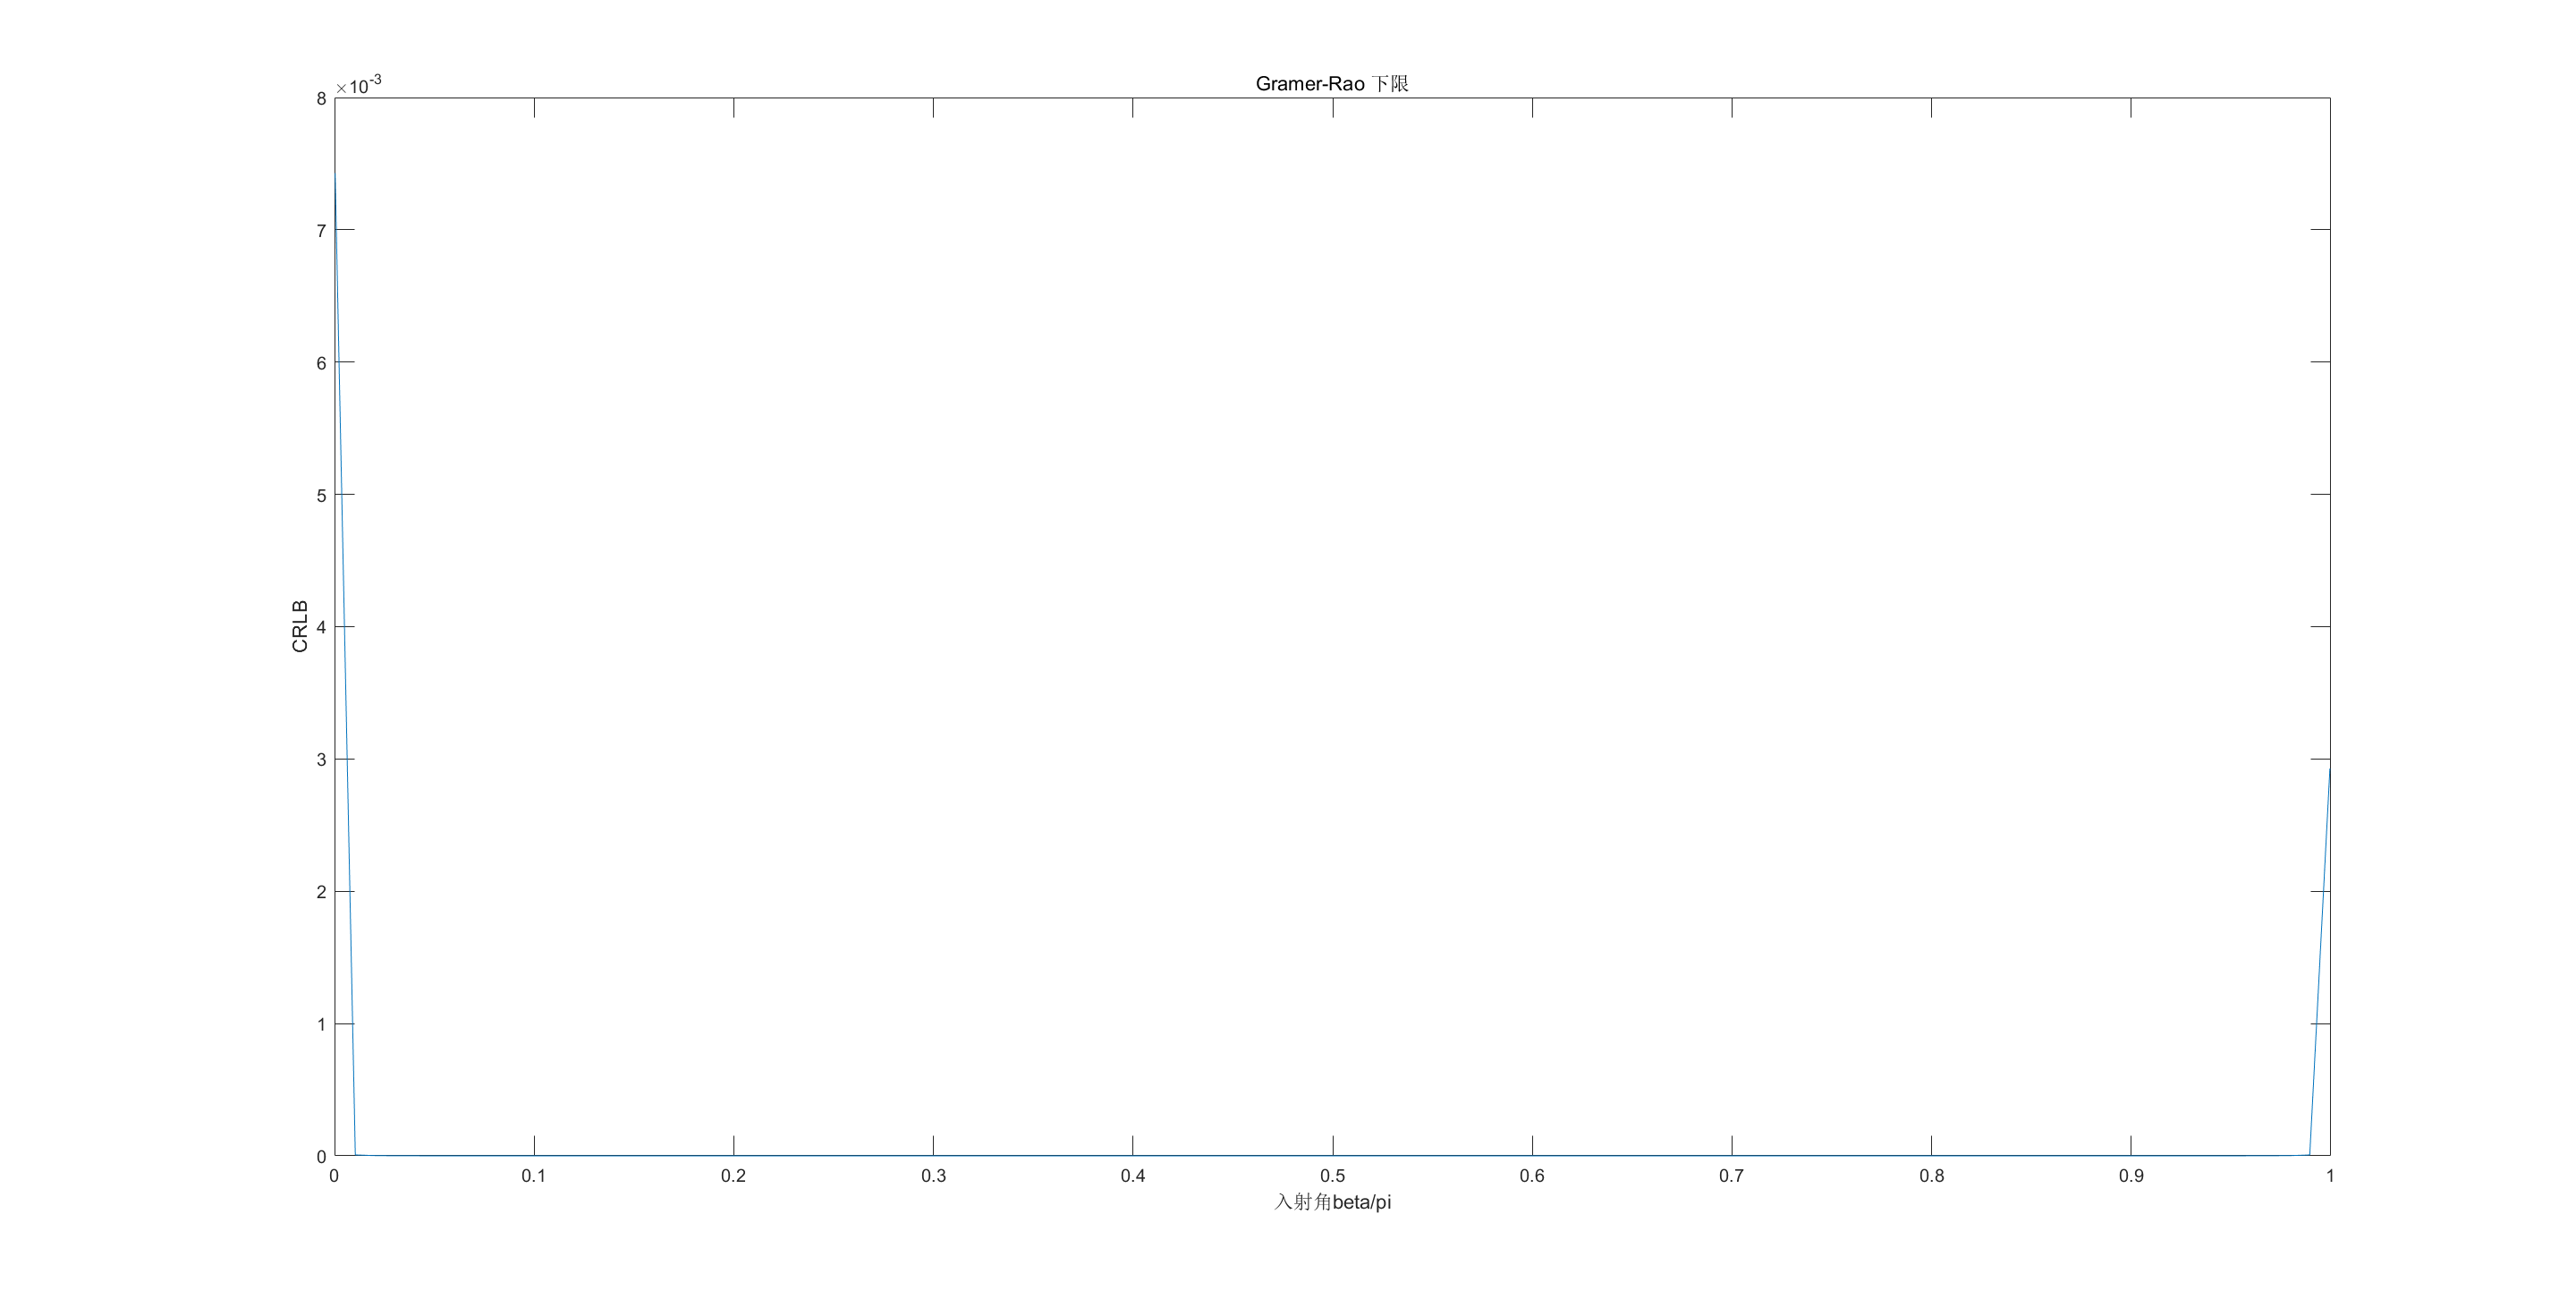
\includegraphics[width=0.75\linewidth]{CRLB 入射角.png}
	\caption{CRLB和入射角之间的关系}
\end{figure}
由图2可知,当$\beta$大于某项值时,CRLB $\to 0$,图像关于$\frac{\pi}{2}$对称,
当$\beta \to 0 或 \pi 时$,CRLB $\to \infty$这是因为靠近入射面时,测量误差很大。
当入射角固定为30°时,设置信噪比$\eta$在[0.001  100]之间变化

\begin{figure}[H]
	\centering
	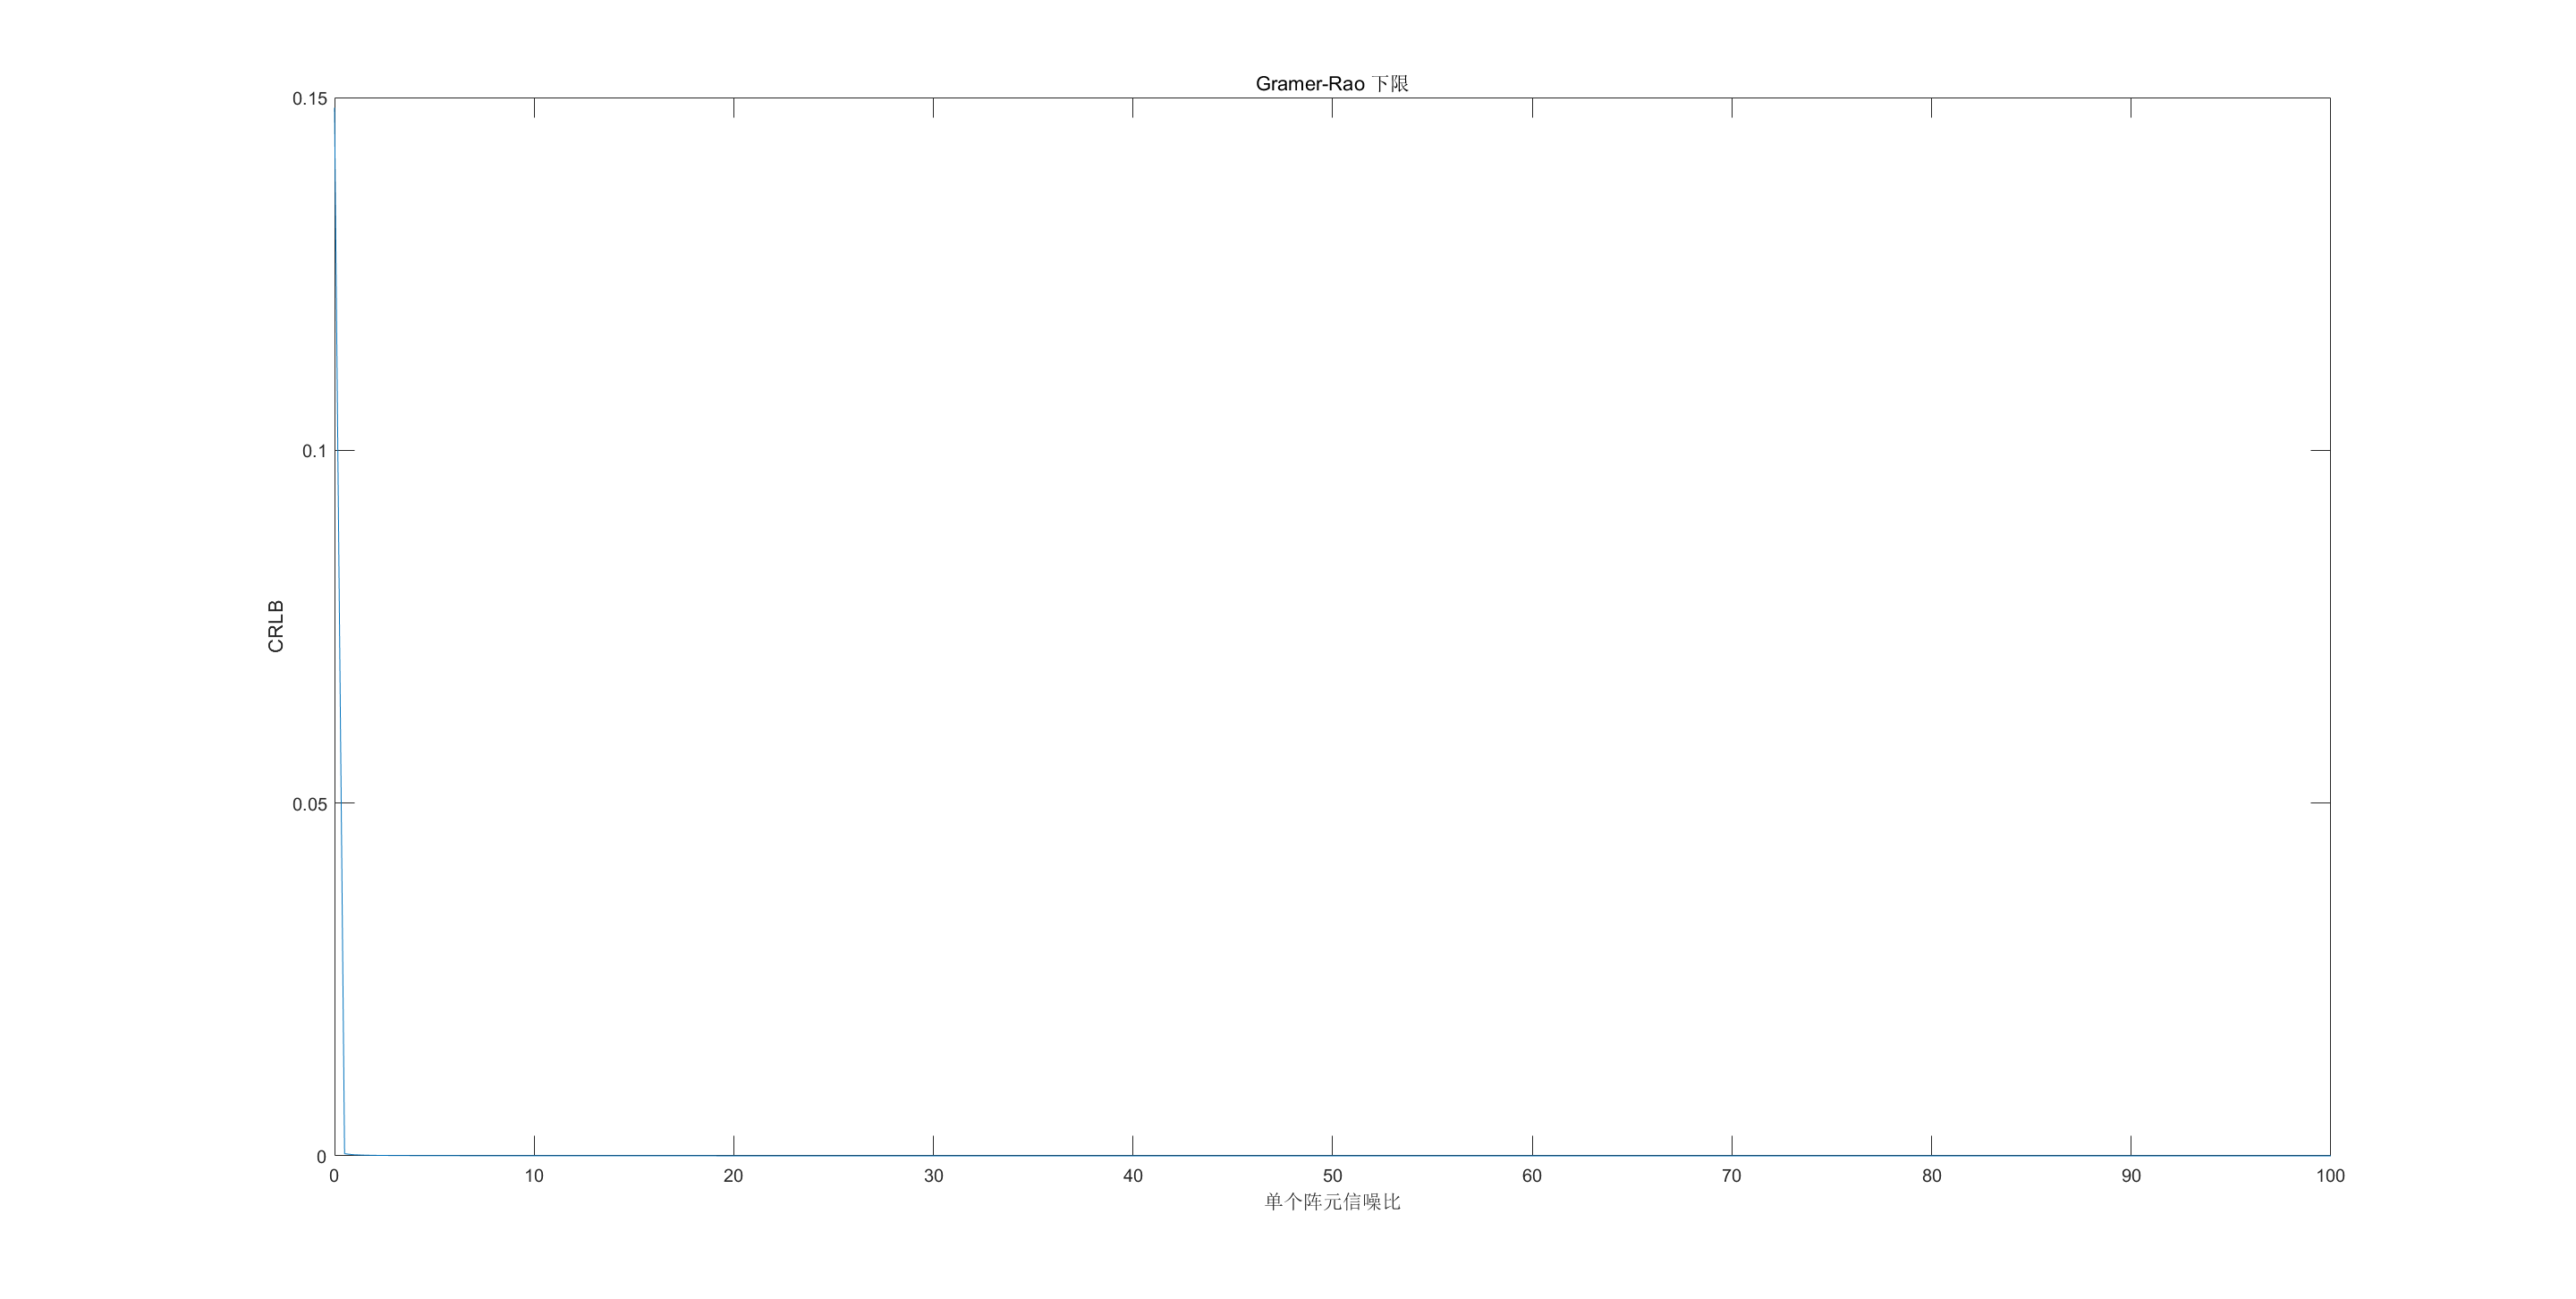
\includegraphics[width=0.75\linewidth]{CRLB 信噪比eta.png}
	\caption{CRLB信噪比$\eta$关系}
\end{figure}
由图像可知,当信噪比$\eta \to \infty$ 时,$CRLB \to 0$,测量误差变小
\begin{itemize}
	\item 设置M从2至50之间变化,入射角固定为30,信噪比$\eta =5dB$时,RLB和入射角之间的关系如下
\end{itemize}
\begin{figure}
	\centering
	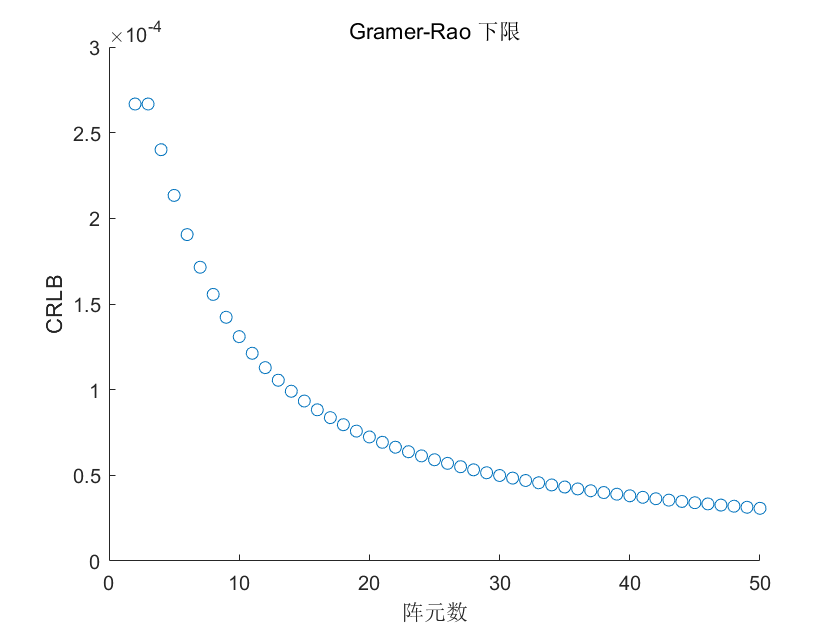
\includegraphics[width=0.75\linewidth]{CRLB 阵元数.png}
	\caption{CRLB和阵元M之间关系}


\end{figure}
由图4.3可知,当阵元数$M$增加 时,$CRLB$减小,且在阵元为2时,即$CRLB$小于0
\begin{itemize}
	\item 设置阵元为8,入射角固定为30度时,CRLB和阵元长度与波长之比之间的关系如下
\end{itemize}
\begin{figure}[H]
	\centering
	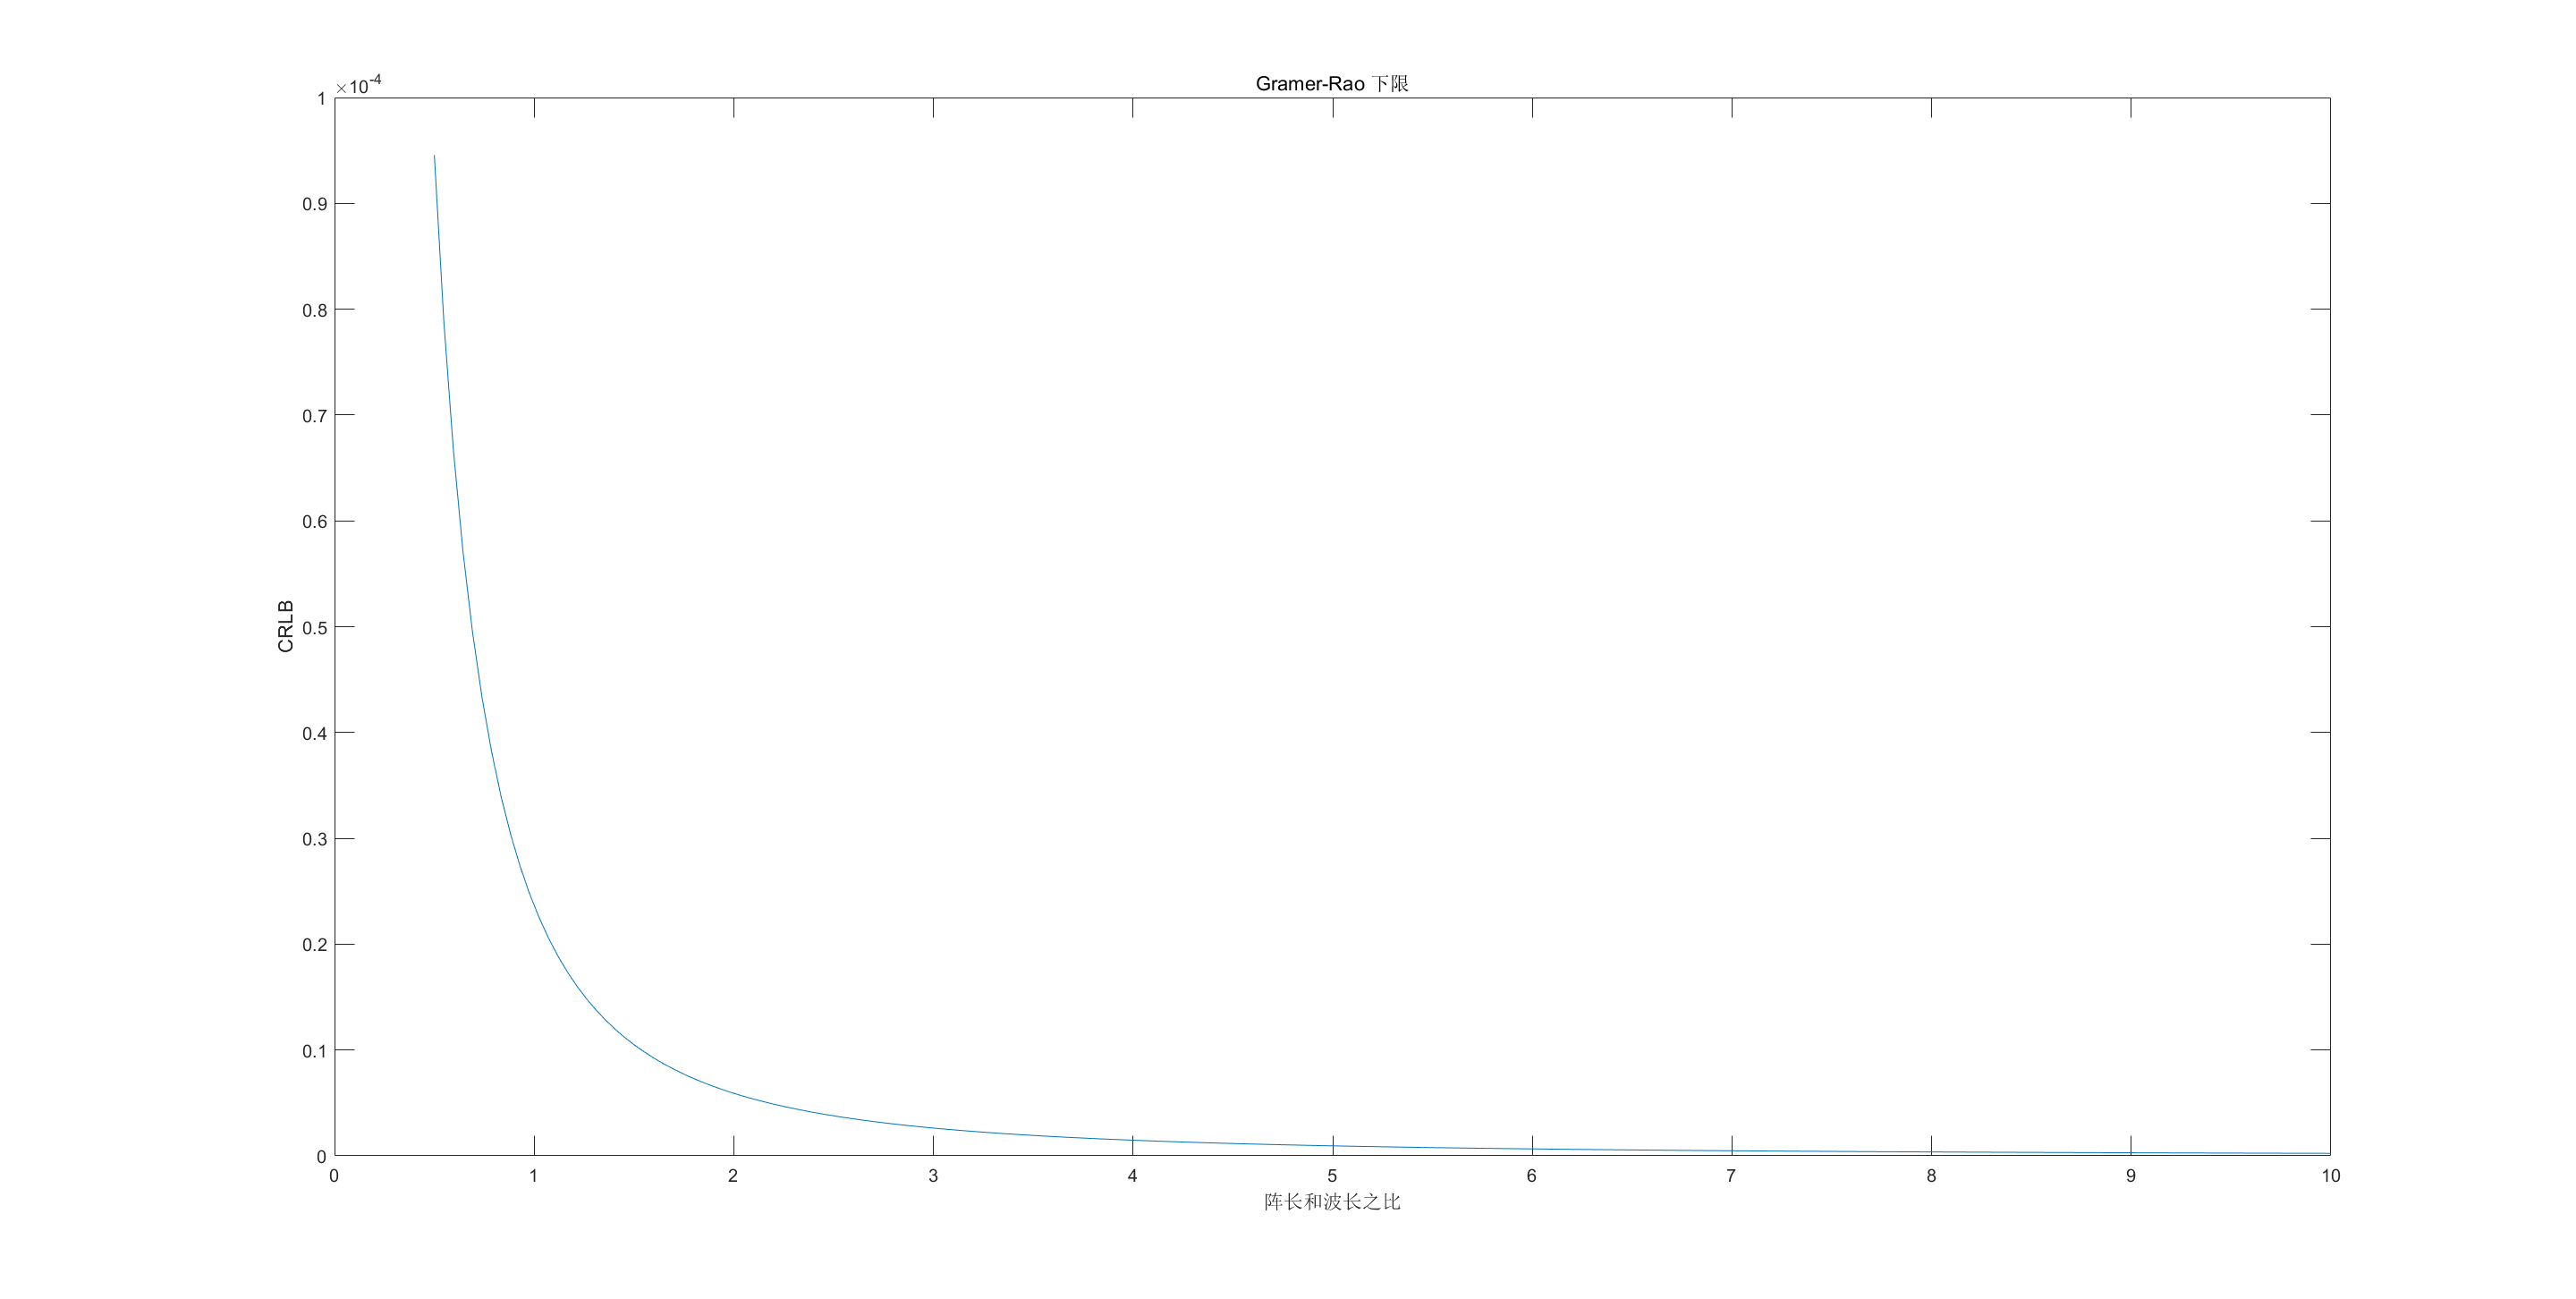
\includegraphics[width=0.75\linewidth]{CRLB 波长比.png}
	\caption{CRLB和阵元长度和波长之比关系}
\end{figure}
有图4.4可知,随着阵元数增加,阵元长和$\lambda$之比增加,$CRLB减少$

\subsection*{(2)阵元与信噪比讨论}

相对阵面入射角度 $\beta=\frac{\pi}{6}$,
信噪比 $10log(\eta)=5dB$
则$\eta$ =3.1623
$\beta$估计偏差小于1°,即$var(\beta)\leq$1;
有上面讨论和M绘制的关系图发现,M=2即可满足条件。
当$M$=8时,若$var(\beta)$小于1,
则求得$eta$=0.804

\subsection*{(3)阵元间距设置}

若来波为C波段,则中心频率$f_0$在4-8GHz,若使$var(\beta)$,由式4.2可知$F_0$
越大,$d$越大,或$\frac{\lambda}{d}$越小($\lambda$越小,$d$越大),则$var(\beta)$越小,即
$$0<\frac{F_0d}{c}cos\beta=\frac{d}{\lambda}cos\beta<\frac{1}{2}$$
则$d$最大取$\frac{\lambda}{2}$,$\lambda$对应为8Ghz时最小,此时$\lambda$=0.0375m

附:matlab代码
\begin{lstlisting}
close all
%按照题目所给数据设置仿真参数
c=3e8;
f0 = 5e9;%中心频率5G
M = 32;%阵元数32
A=1;
sigma2 = 0.01;
eta= 0.5*A^2/sigma2^2; %信噪比
beta=linspace(0.001,3.14,100);%入射角
lambda = c/f0;%入射信号波长
d = 0.5*lambda; %孔径间距
L_lambda = (M-1)*d/lambda;%L/lambda 之比,L阵的长度(M-1)d

%CRLB of beta 入射角的CRLB 
y1=4*pi^2*M*eta*(M+1)/(M-1)*L_lambda^2.*sin(beta).^2;
y=12./y1;
%绘制CRLB和入射角之间的图形
figure(1)
plot(beta/pi,y)
xlabel('入射角beta/pi');
ylabel('CRLB');
title('Gramer-Rao 下限')

%%当入射角为60度(相对阵面方向为30度)时CRLB和信噪比eta 的关系
beta=pi/6;%入射角为30°
eta=linspace(0.001,100,200);
y1=4*pi^2*M*eta*(M+1)/(M-1)*L_lambda^2.*sin(beta).^2;
y=12./y1;
figure(2)
plot(eta,y);
xlabel('单个阵元信噪比');
ylabel('CRLB');
title('Gramer-Rao 下限')

%%当入射角为60度(相对阵面方向为30度)时CRLB和阵元数量M 的关系
beta=pi/6;%相对阵面方向为30度
M = 2:1:50;
eta=3.1623%信噪比即为5dB;
y1=4*pi^2.*M*eta.*(M+1)./(M-1)*L_lambda^2.*sin(beta).^2;
y=12./y1;
figure(3)
scatter(M,y);
xlabel('阵元数');
ylabel('CRLB');
title('Gramer-Rao 下限')

%%当入射角为60度(相对阵面方向为30度)时CRLB和阵的长度和波长之比L_lambda 的关系
beta=pi/6;%入射角设定为30°
L_lambda=linspace(0.5,15,200);
eta= 0.5*A^2/sigma2^2; %信噪比
M=8;
y1=4*pi^2*M*eta*(M+1)/(M-1).*L_lambda.^2.*sin(beta).^2;
y3=12./y1;
figure(4)
plot(L_lambda,y3);
xlabel('阵长和波长之比');
ylabel('CRLB');
title('Gramer-Rao 下限')
\end{lstlisting}

\bibliography{books}
\end{document}